\chapter{Experimentação e resultados}
\label{cap:experiments}

\section{Ambiente de simulação}

Uma simulação da rede nacional de pesquisa, a rede Ipê \citep{ipe2015network} 
foi criada em laboratório.
Um comutador (\emph{switch}) OpenFlow e quatro servidores foram utilizados 
para executar a simulação no laboratório WiNet \citep{winet22015lab}
no departamento de Ciência da Computação (DCC) da Universidade Federal 
de Minas Gerais (UFMG).

\subsection{A rede Ipê}
Operada pela Rede Nacioanal de Pesquisa (RNP), a rede Ipê é uma infraestrutura
de rede Internet dedicada à comunidade de pesquisa brasileira.
Inaugurada em 2005, foi a primeira rede óptica nacional acadêmica a entrar em
operação na América Latina.

A rede IPÊ implementa 27 Pontos de Presença (\emph{POPs}), um para cada unidade
da federação.
Em cada unidade existem diversos clientes que, para se comunicar com outras 
máquinas em outros Pontos de Presença, transmitem seus pacotes através do 
POP ao qual atuam como clientes.
Essas ramificações constituem mais de 800 instituições de ensino, saúde e 
pesquisa em todo o país, beneficiando mais de 3,5 milhões de usuários
\citep{ipe2015network}.

Através da rede RedCLARA \citep{redclara2015network}, a rede Ipê se conecta 
à 2,5 Gb/s com, atualmente, 15 países da América Latina e à 5 Gb/s com a rede
europeia Géant \citep{geant2015network}. 
Além disso, por meio de quatro conexões de
10 Gb/s, duas pelo Oceano Atlântico e duas pelo Oceano Pacífico, 
operadas em parceria com a ANSP, totalizando 40 Gb/s, a rede Ipê se conecta 
às redes acadêmicas norte-americanas, em especial, a  Internet2 
\citep{internet22015network}, a outras redes acadêmicas internacionais e à 
internet comercial mundial.

Os Pontos de presença estão interconectados conforme mostrado na figura 
\ref{fig:ipe-network-2015}.

\begin{figure}[!ht]
    \centering
    \label{fig:ipe-network-2015}
    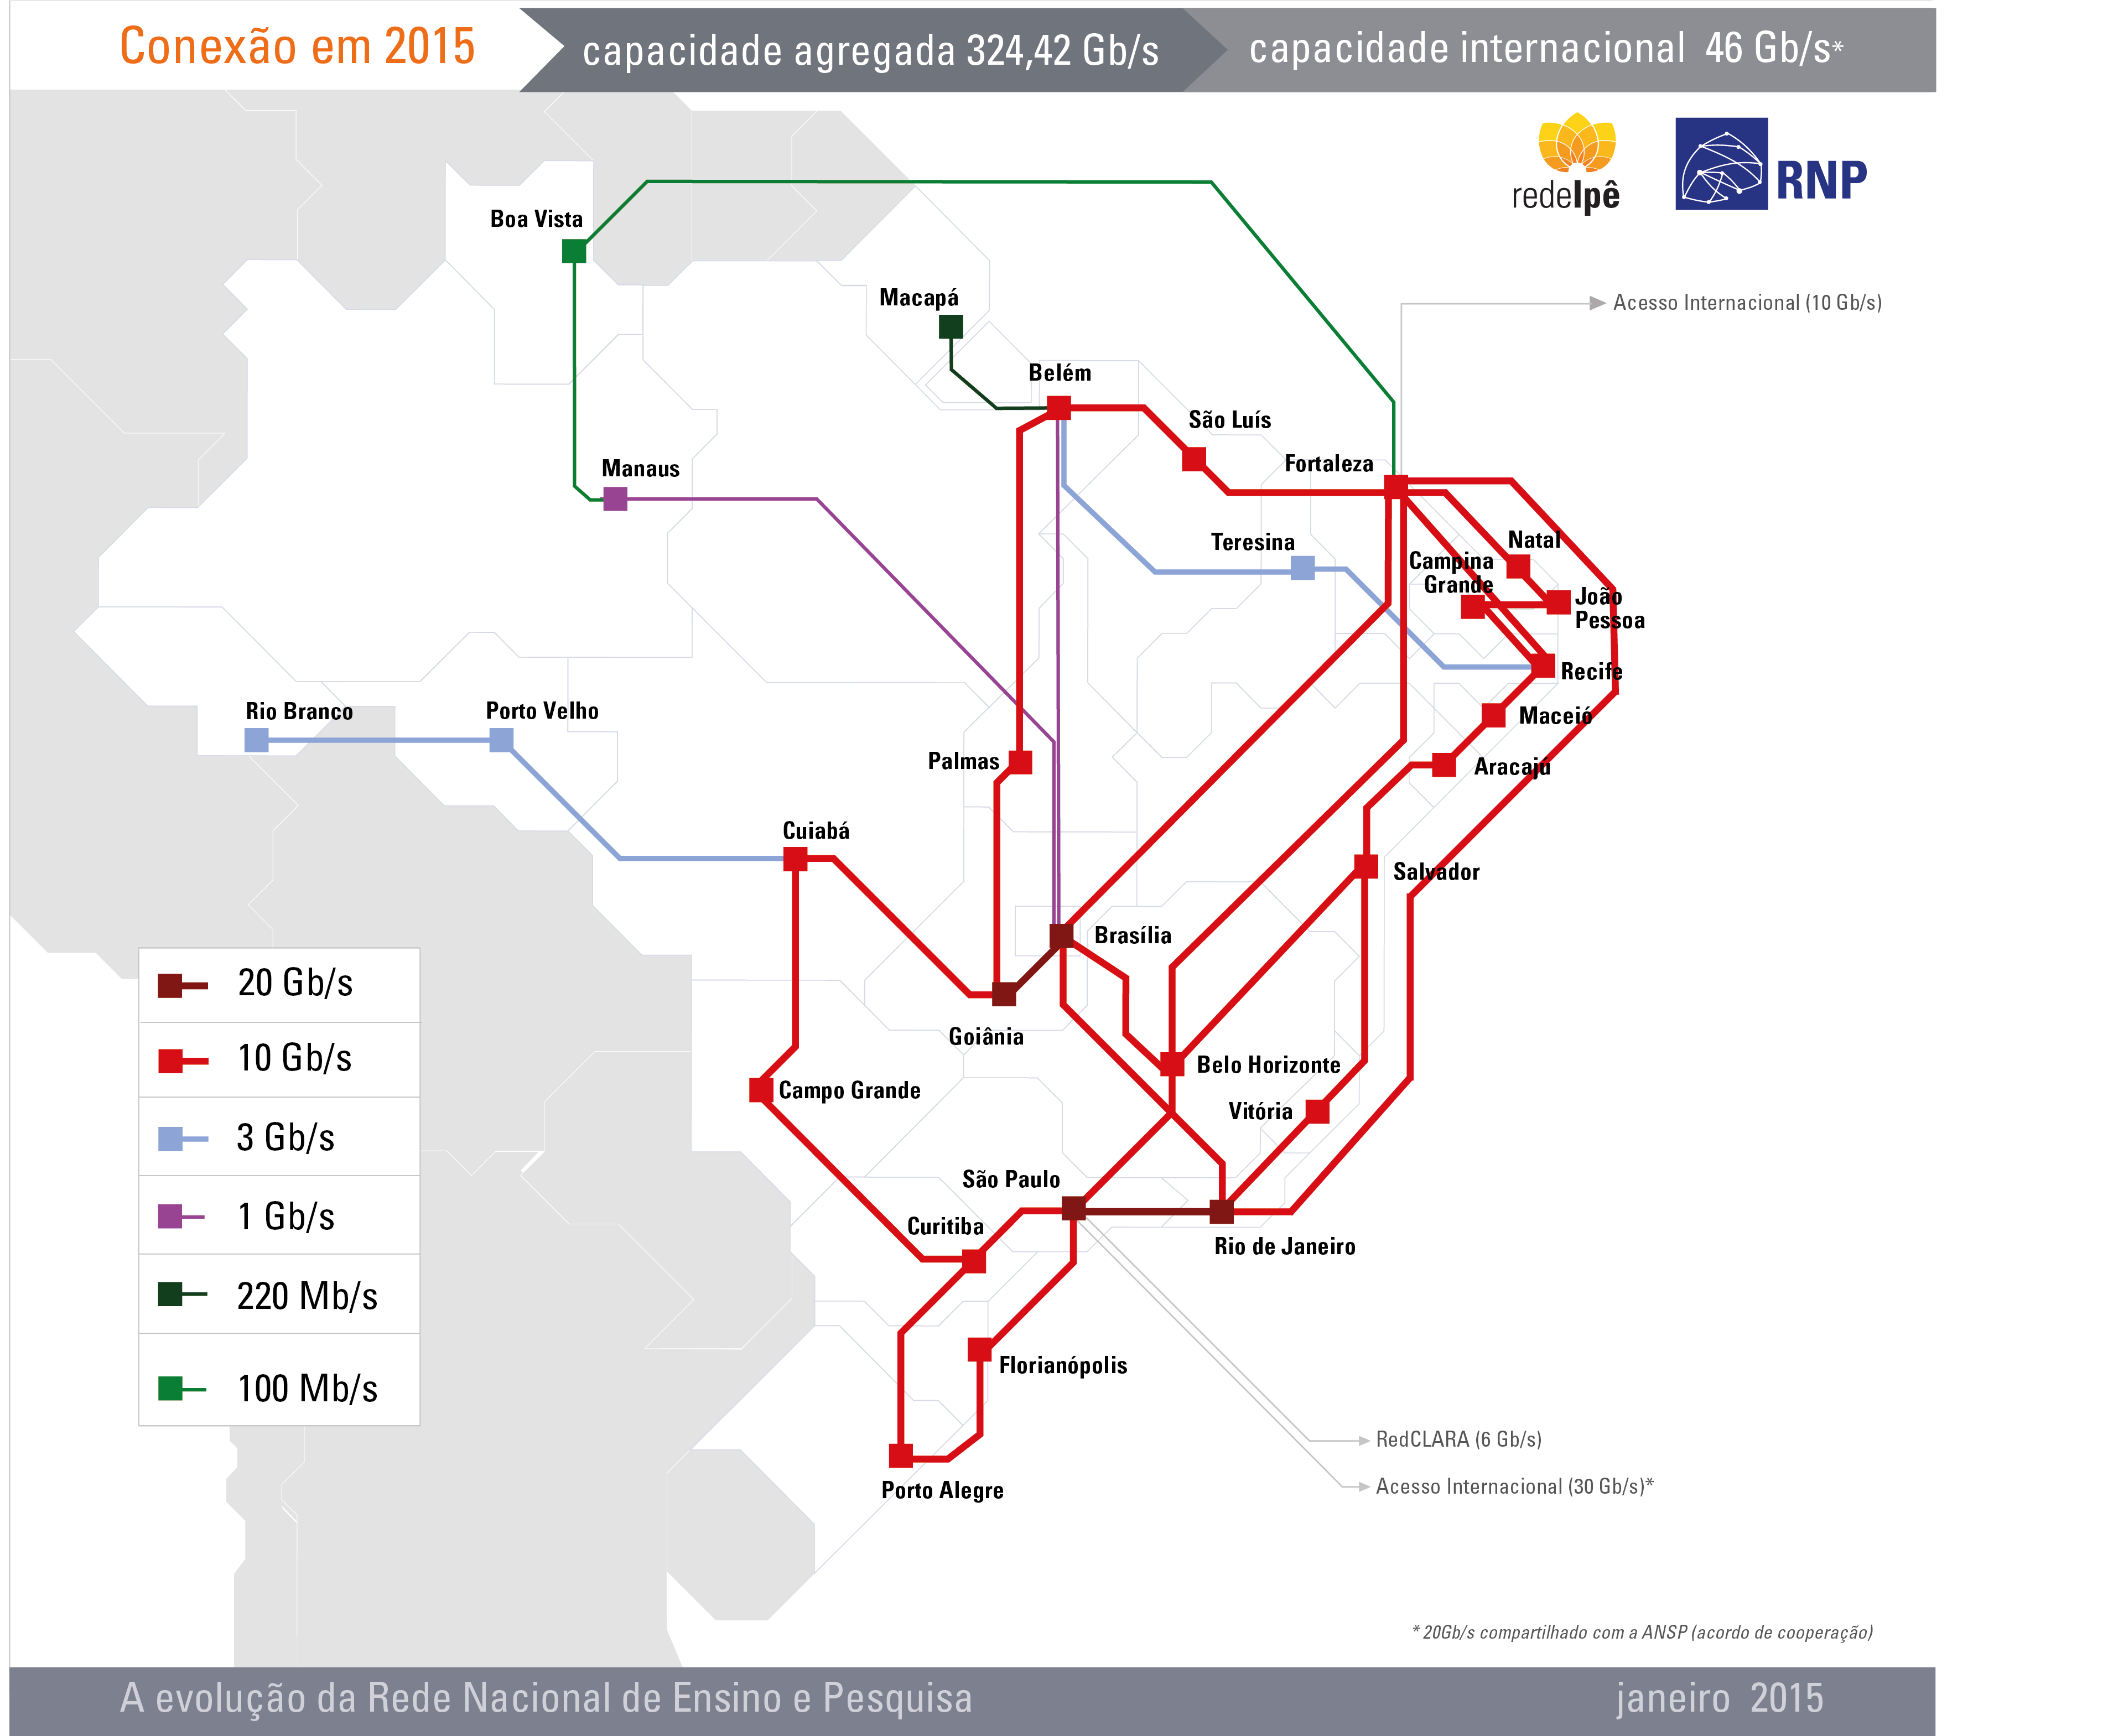
\includegraphics[width=\textwidth]{img/ipe-network-2015}
    \caption{Rede Nacional de Pesquisa IPÊ \protect\footnotemark}
    \vspace*{3in}
\end{figure}

\footnotetext{Imagem retirada de 
\url{http://www.rnp.br/servicos/conectividade/rede-ipe}}

\subsection{Arquitetura da simulação}

A ambiente de simulação é composto por um comutador HP com OpenFlow habilitado.
Quatro servidores são responsáveis por gerenciar máquinas virtuais que 
representam as unidades federativas e suas instituições clientes.

Conforme pode ser visto na figura \ref{fig:physical-vs-virtual-network}, a
rede física do esperimento é separada da rede virtual.
O quinto computador é o controlador da rede. 
Para o experimento, existem duas redes. 
Uma rede de administração, com acesso aos servidores e a uma instância do 
controlador, na porta 6633.
A segunda rede é a rede virtual à qual todos os POPs simulados estão 
conectados. 
Para implementar essas duas redes, cada servidor e o controlador possuem duas
interfaces de rede que isolam seus funcionamentos.
Assim, a rede física/administrativa e a rede virtual/Ipê estão separadas
em nosso experimento.


\begin{figure}[!h]
    \centering
    \label{fig:physical-vs-virtual-network}
    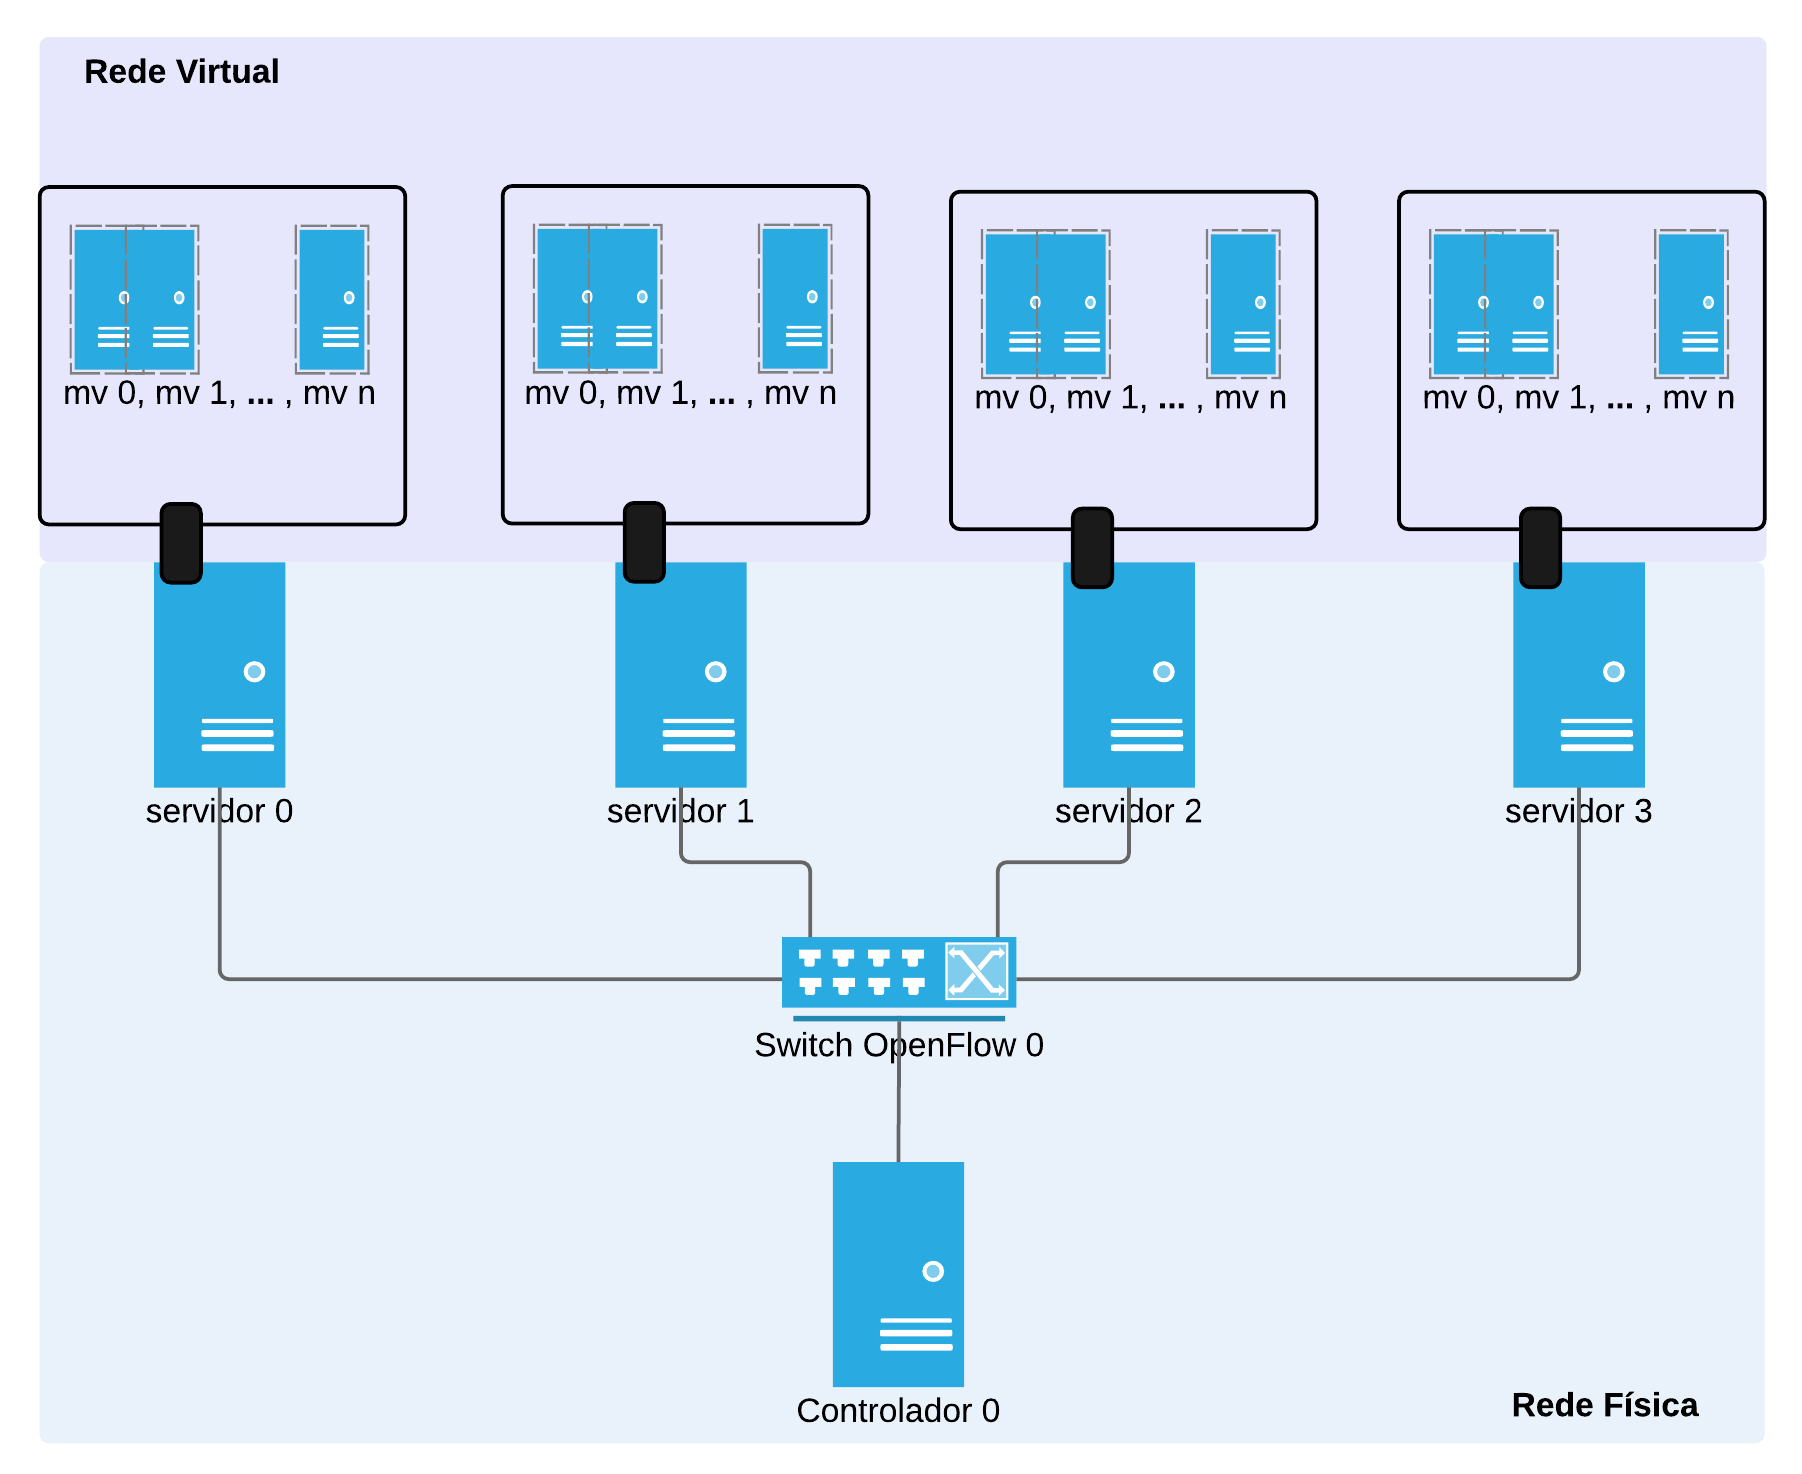
\includegraphics[width=\textwidth]{img/physical-vs-virtual-network-pt}
    \caption{Arquitetura do ambiente de simulação}
\end{figure}

Para o ambiente virtualizado, o controlador está associado a porta 6653.
Cada POP é um comutador (\emph{switch}) OpenFlow simulado via OpenVSwitch
\citep{openvswitch2015switch}.
As instituições clientes de cada POP são simuladas através do \emph{Mininet} 
\citep{lantz2010network}.
O número de instituições clientes foi coletado do sítio de cada Ponto de 
Presença.

Cada máquina virtual representa um POP.
Cada POP possui uma subrede à qual uma instância do \emph{Mininet} simula 
seus clientes. 
Essa subrede está conectada através de um \emph{switch} virtual 
\emph{OpenVSwitch} que é controlado pelo controlador da rede virtualizada.
Assim, para cada POP, temos as decisões e atualizações da tabela de fluxos
feita pelo controlador.
Toda comunicação de saída das subredes utilizando \emph{mininet} passam pelo 
\emph{OpenVSwitch} que funciona em modo \emph{bridge} (ponte) com a interface
de rede virtual conforme pode ser visto na figura
\ref{fig:mininet-vm-architecture}.


\begin{figure}[h!]
    \centering
    \label{fig:mininet-vm-architecture}
    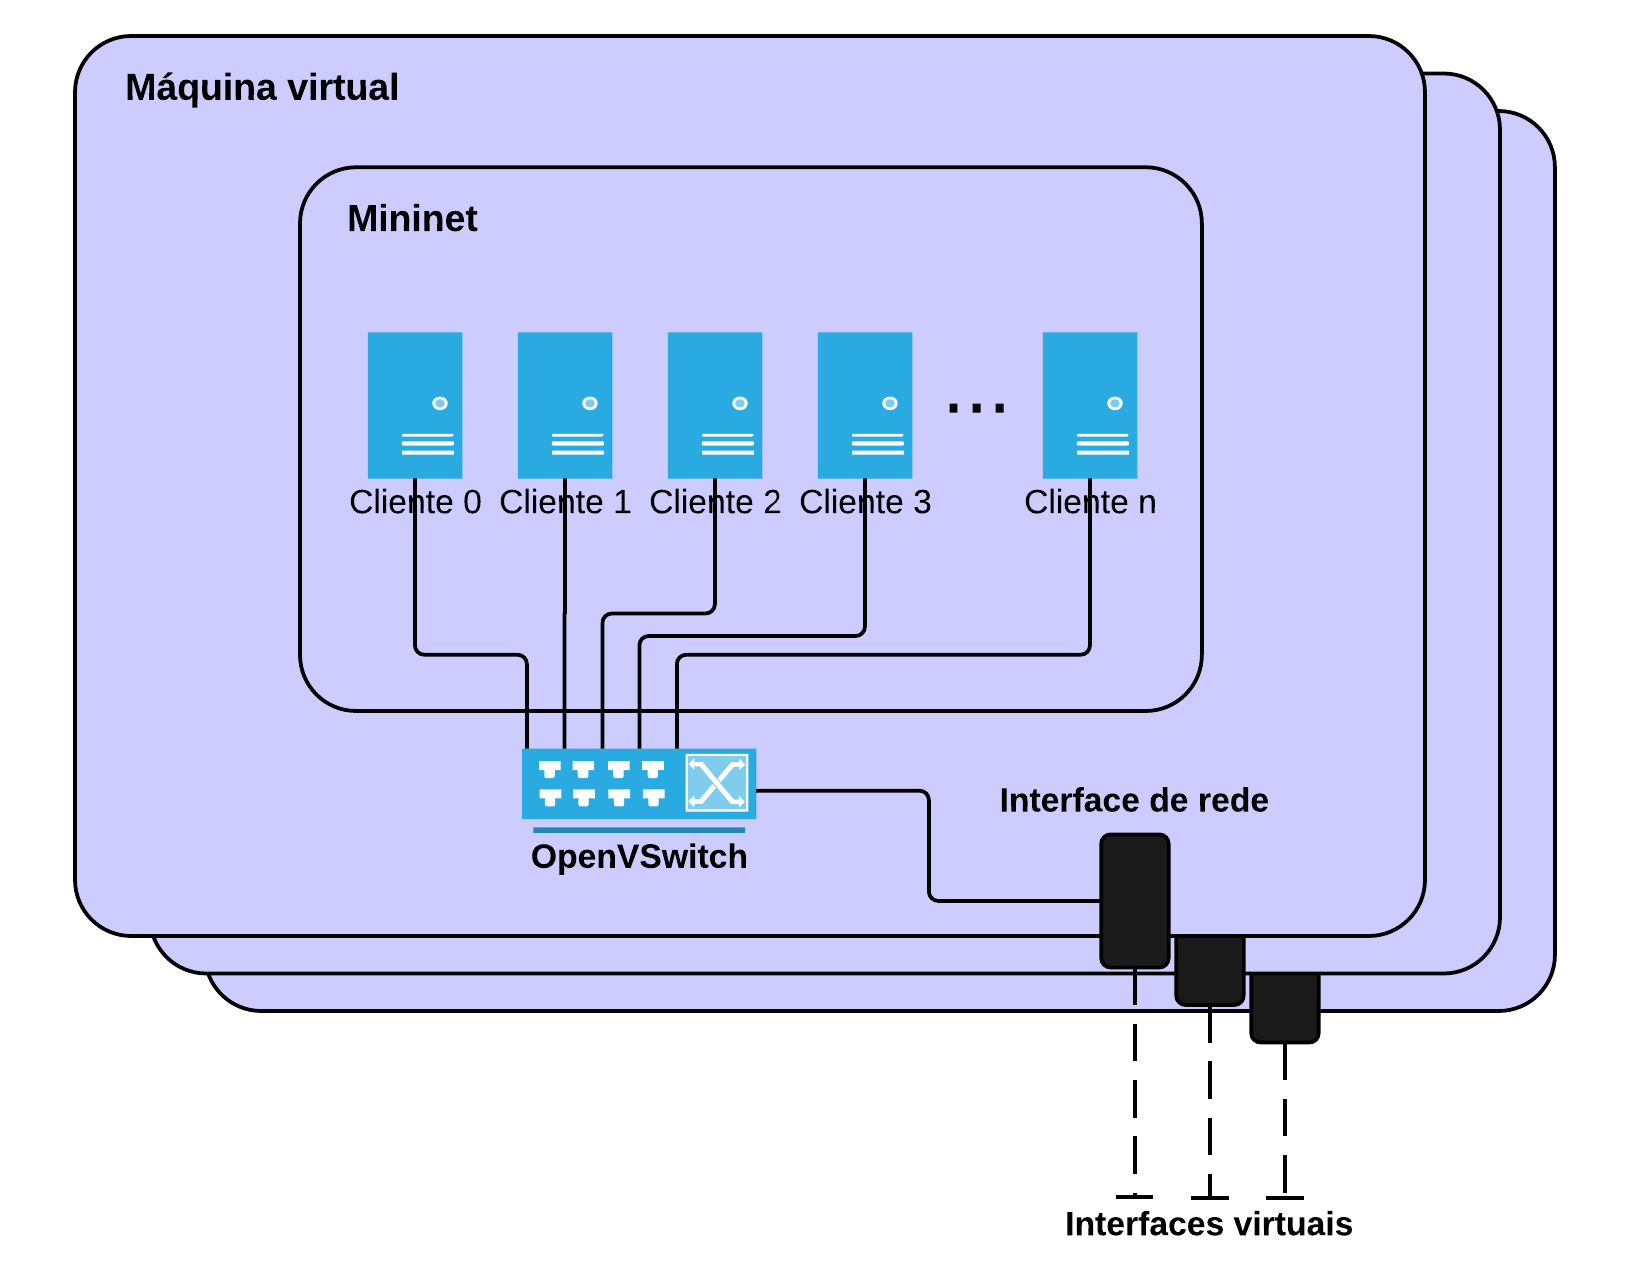
\includegraphics{img/mininet-vm-architecture}
    \caption{Arquitetura de cada máquina virtual}
\end{figure}


A tabela \ref{tbl:testbed-ipe-net} apresenta as subredes de cada unidade
federativa (POP), qual servidor físico gerencia a máquina virtual referente
ao POP e o número de clientes a ele associado.

\begin{table}[h]
    \label{tbl:testbed-ipe-net}
    \centering
    \resizebox*{!}{\dimexpr\textheight- 25px}{
    \resizebox{\linewidth}{!}{
    \begin{tabular}{llllll}
        \rowcolor[HTML]{000000} 
        \multicolumn{6}{c}{\cellcolor[HTML]{000000}{\color[HTML]{C0C0C0} 
            \textbf{Associação de Servidores à simulação da rede IPÊ}}} \\
        \rowcolor[HTML]{000000} 
        {\color[HTML]{9B9B9B} \textbf{UF}} & {\color[HTML]{9B9B9B} 
            \textbf{N clientes}} & {\color[HTML]{9B9B9B} 
            \textbf{Sub-rede local}} & {\color[HTML]{9B9B9B} 
            \textbf{Servidor}} & {\color[HTML]{9B9B9B} \textbf{IP local}} & 
            {\color[HTML]{9B9B9B} \textbf{IP Gateway}} \\
        AC &  10 &  10.10.1.0 &   Shiva  &  10.10.42.51 & \\ 
        AL  & 13 &  10.10.2.0  &  Shiva  &  10.10.42.52 & \\ 
        AM  & 20 &  10.10.3.0 &   Shiva  &  10.10.42.53 & \\
        AP  & 7  &  10.10.4.0 &   Shiva  &  10.10.42.54 & 10.10.42.50 \\
        BA  & 25 &  10.10.5.0 &   Shiva  &  10.10.42.55 & \\
        CE  & 50  & 10.10.6.0  &  Shiva  &  10.10.42.56 & \\
        DF  & 16 &  10.10.7.0  &  Shiva  &  10.10.42.57 & \\ \hline
        ES  & 26  & 10.10.8.0  &  Eden  &   10.10.42.101 & \\
        GO  & 26  & 10.10.9.0  &  Eden  &   10.10.42.102  & \\  
        MA  & 7  &  10.10.10.0 &  Eden  &   10.10.42.103  & \\  
        MG  & 32  & 10.10.11.0  & Eden  &   10.10.42.104  & 10.10.42.100 \\  
        MS  & 10  & 10.10.12.0  & Eden  &   10.10.42.105  & \\  
        MT  & 8   & 10.10.13.0  & Eden  &   10.10.42.106  & \\  
        PA  & 13  & 10.10.14.0  & Eden  &   10.10.42.107  & \\ \hline
        PB  & 14  & 10.10.15.0  & Diablos & 10.10.42.151  & \\
        PE  & 41  & 10.10.16.0  & Diablos & 10.10.42.152  & \\  
        PI &  25 &  10.10.17.0 &  Diablos & 10.10.42.153  & \\  
        PR &  71 &  10.10.18.0 &  Diablos & 10.10.42.154  & 10.10.42.150 \\
        RJ &  27 &  10.10.19.0 &  Diablos & 10.10.42.155  & \\  
        RN &  11 &  10.10.20.0 &  Diablos & 10.10.42.156  & \\  
        RO &  10 &  10.10.21.0 &  Diablos & 10.10.42.157  & \\ \hline
        RR  & 7  &  10.10.22.0 &  Leviathan &   10.10.42.201 & \\
        RS &  10 &  10.10.23.0 &  Leviathan &   10.10.42.202  & \\  
        SC &  47 &  10.10.24.0 &  Leviathan &   10.10.42.203 & 10.10.42.200 \\   
        SE &  13 &  10.10.25.0 &  Leviathan &   10.10.42.204 & \\   
        SP &  25 &  10.10.26.0 &  Leviathan &   10.10.42.205  & \\  
        TO &  11 &  10.10.27.0 &  Leviathan &   10.10.42.206 & \\   
    \end{tabular}
    }}
\end{table}



\section{Detecção de entidades}

Ao ser carregado, o módulo \emph{graph} inicia o grafo da rede vazio.
Os \emph{switches} são os primeiros a serem identificados. 
Como o controlador está ligado diretamente a eles pela interface
\emph{OpenFlow}, um evento de \emph{ConnectionUp} é disparado 
pelo núcleo do controlador.
Esse evento dispara o evento \emph{SwitchJoin} através do módulo 
\emph{topology} que faz com que o grafo adicione vértices.

\begin{figure}[h!]
    \centering
    \begin{lstlisting}[ tabsize=4,  
                        language=bash,
                        basicstyle=\ttfamily\footnotesize,
                        aboveskip={1.5\baselineskip},
                        columns=fixed,
                        showstringspaces=false,
                        extendedchars=true,
                        breaklines=true,
                        frame=single,
                        numbers=left,
                        showtabs=false,
                        showspaces=false,
                        showstringspaces=false,
                        identifierstyle=\ttfamily,
                        ]
INFO:topology.graph:SwitchJoin id: 2
INFO:topology.graph:SwitchJoin id: 1
INFO:topology.graph:1, 2
DEBUG:openflow.discovery:Dropping LLDP packet 275
INFO:topology.graph:LinkEvent fired
INFO:host_tracker:Learned 1 1 7e:e6:9b:89:39:2e got IP 10.0.0.1
INFO:topology.graph:HostJoin id: 7e:e6:9b:89:39:2e
INFO:host_tracker:Learned 2 1 62:77:44:24:13:49 got IP 10.0.0.2
INFO:topology.graph:HostJoin id: 62:77:44:24:13:49
        \end{lstlisting}
    \caption{Detecção de entidades}
    \label{fig:detection}
\end{figure}

Nas duas primeiras linhas do \emph{log} mostrado na figura
\ref{fig:detection}, o módulo \emph{graph} foi notificado
da descoberta de dois \emph{switches} na rede.
Na linha 5, nota-se a descoberta de um enlace (\emph{link}) entre dois
comutadores (\emph{switches}).
O módulo \emph{openflow.discovery}, através do protocolo LLDP identificou 
o link entre \emph{switches}.
O grafo foi notificado e estabeleceu uma aresta entre os 
vértices (\emph{switches}).

As linhas 7 e 9 mostram a descoberta de dois hosts.
Esses hosts foram descobertos pelo módulo \emph{host\_tracker} via 
escuta dos eventos de DHCP.
É importante ressaltar que a descoberta de \emph{hosts} também ocorre 
independente do DHCP.
Um novo pacote que passa por um \emph{switch} e não possui regra
instalada na tabela de fluxos é encaminhado ao controlador que 
dispara um evento de \emph{PacketIn}. 
Para tal, o \emph{host\_tracker} se encarrega de escutar esse evento 
e notificar o grafo através do evento \emph{HostJoin} disparado pelo módulo
\emph{topology} ao criar um novo \emph{Host}.
O grafo, ao ser notificado, cria vértices para esses \emph{hosts} associando 
uma aresta entre eles e o \emph{switch} ao qual eles estão conectados.
Dessa forma as entidades da rede são identificadas e computadas no grafo.


\section{Remoção de entidades}

Diversos computadores foram desligados de maneira aleatória.
O \emph{host\_tracker}, após um tempo fixo (\emph{timerInterval}) 
verifica via ARPPing se os \emph{hosts} conhecidos estão ativos.
Para esse cenário da remoção de um computador (\emph{host}), 
o \emph{host\_tracker} identifica a inatividade do \emph{host} e remove o 
\emph{Host}.
O evento de \emph{HostLeave} é disparado pelo \emph{topology}, 
atualizando assim o grafo.

Nesse cenário de experimento, cinco computadores de cada subrede foi desligado.
Para cada computador foi coletado o tempo em que ele foi desligado.
Quando o controlador, através do \emph{host\_tracker}, identifica a saída 
desse computador o tempo é novamente coletado.
Assim, para cada computador desligado, foi computado o tempo decorrido até 
que o controlador o removesse do grafo da rede.

\begin{figure}[h!]
    \centering
    \label{fig:hosts-leave-time}
    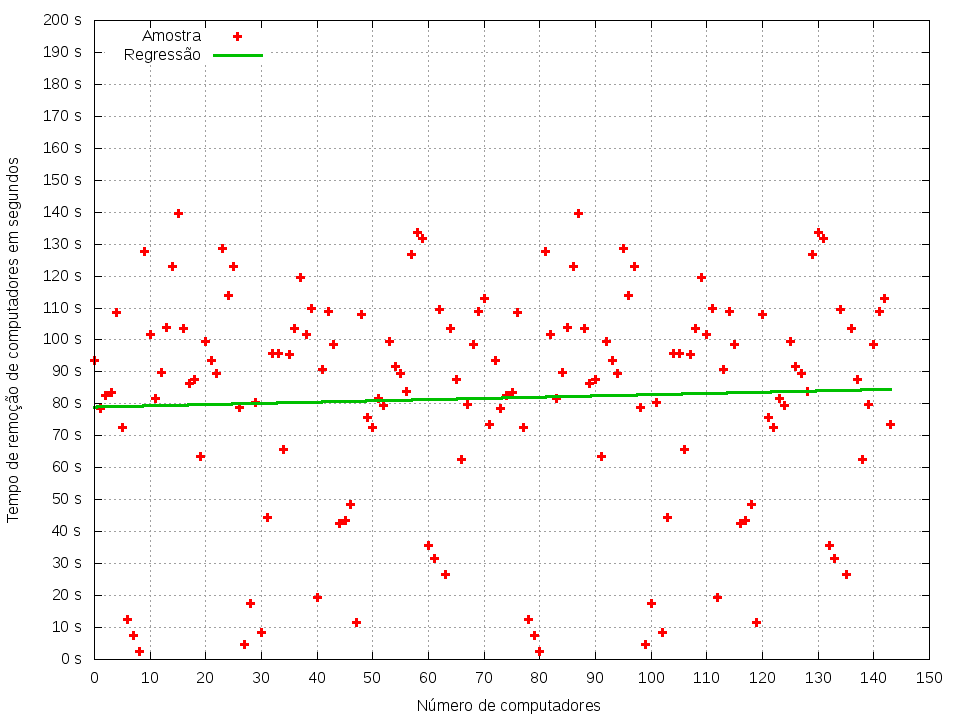
\includegraphics[width=\linewidth]{img/hosts-leave-time}
    \caption{Tempo decorrido entre o desligamento de um computador e a 
    remoção do mesmo no grafo}
\end{figure}

Os resultados da amostra coletada pode ser visto na figura
\ref{fig:hosts-leave-time}.
Em média, o tempo de remoção de um computador do grafo demorou 80 segundos.
A sondagem foi configurada para ser executada com uma periodicidade de 60 
segundos. 
A regressão linear computada mostra que esse valor médio é praticamente 
constante ao longo dos valores amostrados.

Computadores cuja remoção ocorreram em um intervalo de tempo muito reduzido
tiveram seu tempo de sondagem expirado muito próximos ao momento em que 
o \emph{host\_tracker} executava sua sondagem. 

Para o caso de comutadores (\emph{switch}), foram desligados os 
\emph{switches} e medido o tempo de atualização do grafo.
O controlador está ligado diretamente aos \emph{switch}. 
Em função disso os comutadores são removidos mais rapidamente do grafo.
A figura \ref{fig:switch-leave-time} apresenta os resultados da 
computação da amostra de \emph{switches} removidos.
Assim, ao ser desligado, o \emph{core} do POX dispara um evento 
de \emph{SwitchLeave} ao qual o módulo \emph{graph} está inscrito. 
Logo, o grafo é atualizado removendo o vértice do \emph{switch}.

\begin{figure}[h!]
    \centering
    \label{fig:switch-leave-time}
    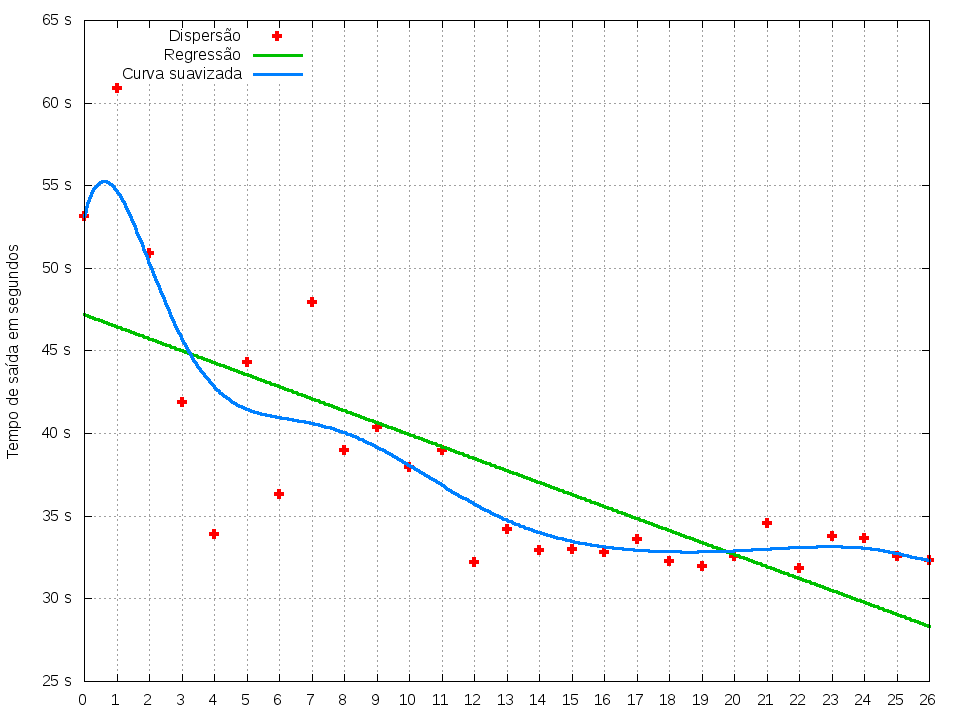
\includegraphics[width=\linewidth]{img/switch-leave-time}
    \caption{Tempo decorrido entre o desligamento de um comutador 
    (\emph{switch}) e a remoção do mesmo no grafo}
\end{figure}

Uma curva suavizada da interpolação dos pontos mostra que apesar dos valores
de tempo mais elevados nos primeiros valores da amostra, ao final esses valores
são praticamente constantes, em um valor de 30 a 35 segundos para cada 
remoção.

Após algum tempo o \emph{host\_tracker} identifica se os computadores 
associados ao \emph{switch} removido estão ativos por outra rota. 
Caso negativo, os computadores são removidos do grafo.
Considerando o experimento da remoção dos comutadores (\emph{switches}),
foi computado o tempo decorrido entre a remoção do \emph{switch} e a 
remoção dos computadores na rede interna ao \emph{switch}. 

\begin{figure}[h!]
    \centering
    \label{fig:hosts-behind-switch-time}
    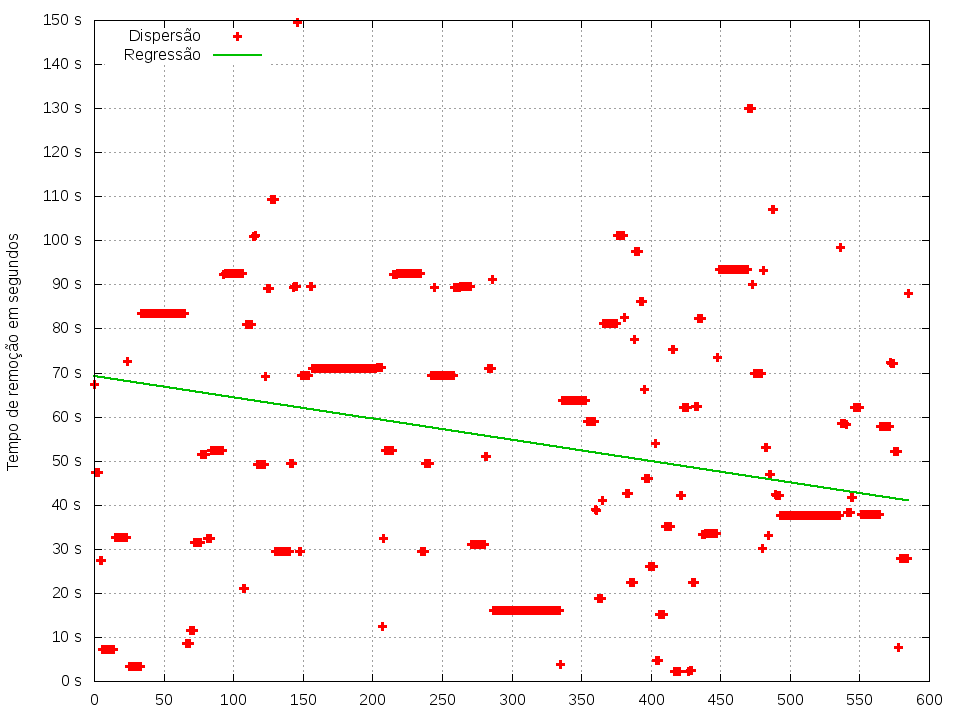
\includegraphics[width=\linewidth]{img/hosts-behind-switch-time}
    \caption{Tempo decorrido entre a remoção dos comutadores 
    (\emph{switches}) e a remoção dos computadores na rede interna ao 
    \emph(switch)}
\end{figure}

A figura \ref{fig:hosts-behind-switch-time} mostra o resultado do experimento
para o tempo de remoção de computadores em função da remoção do 
\emph{switch}.
Os resultados mostram uma média que varia entre 40 e 70 segundos para a 
remoção dos computadores.
No geral nota-se que computadores de uma mesma subrede foram removidos em 
instantes próximos.
Isso pode ser notado pelos pequenos grupos de pontos muito próximos na 
figura.

\section{Visualização em tempo real}

Em um intervalo predefinido, uma imagem representando o grafo atual da rede
é gerada pelo módulo \emph{graph}.
Um exemplo de grafo é apresentado na figura \ref{fig:full-graph}.
Esse grafo representa uma rede simulada, dentro do ambiente do 
\emph{Mininet}, com 8 comutadores (\emph{switches}), cada um com 30 
computadores (\emph{hosts}) conectados totalizando 248 entidades na rede.


\begin{figure}[h!]
    \centering
    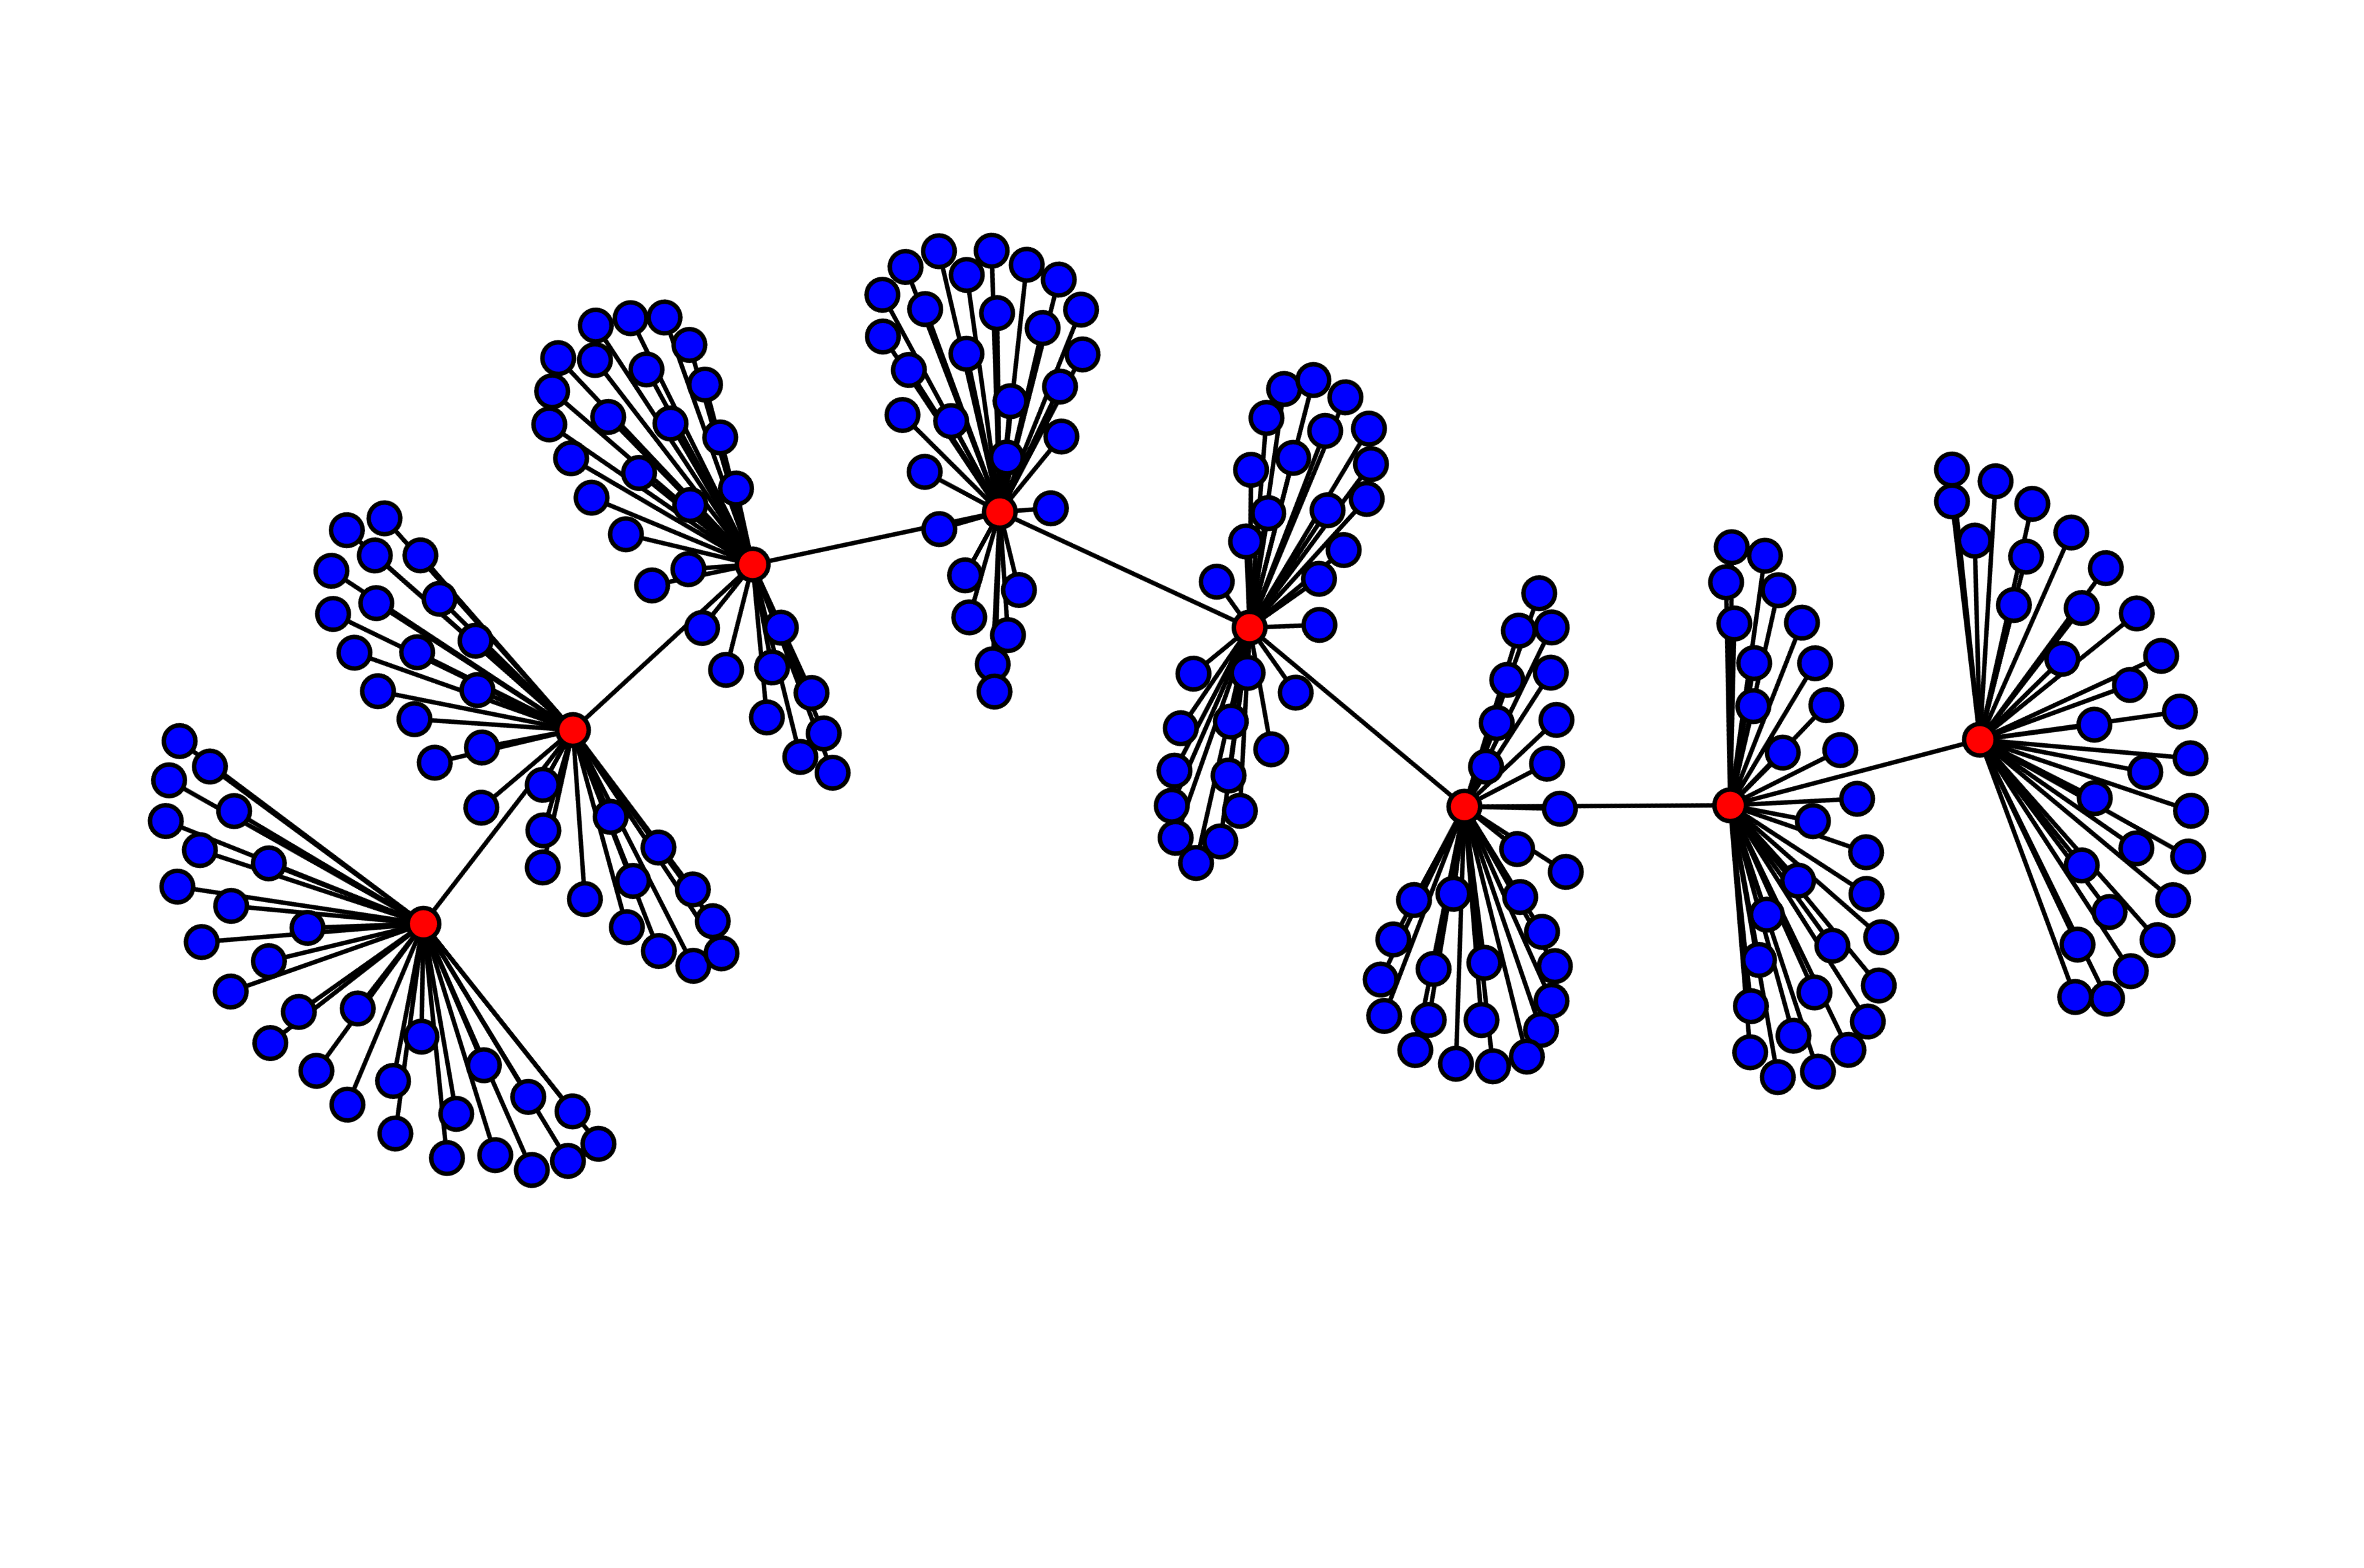
\includegraphics[width=\textwidth]{img/full-graph}
    \caption{Grafo representando uma rede com 248 entidades}
    \label{fig:full-graph}
\end{figure}

Atualizações na topologia como, remover e adicionar entidades na rede, foram
executados.
A visualização da rede atualiza junto com as alterações no grafo.

\section{Identificação de tráfego}

Para computar o tráfego (TCP) em uma rede simples foi executado o programa 
\emph{iperf} como servidor no \emph{host} 'Host 0a'.
A topologia dessa rede é composta por dois comutadores interligados.
Cada comutador possui três computadores em cada subrede.
O \emph{host} 'Host 1e' conecta-se como cliente. 

Conformo pode ser notado na figura \ref{fig:iperf}, o tráfego 
em bytes na arestas desses \emph{hosts} é superior ao demais \emph{hosts}.
No momento em que foram lidos os contadores \emph{OpenFlow} e computados
os pesos das arestas, obteve-se um tráfego de 55894 bytes através do caminho
entre os dois \emph{hosts} citados.
Os valores apresentados para os demais \emph{hosts} (41 bytes) são referentes
ao tráfego ARP PING disseminado pelo módulo \emph{host\_tracker}

\begin{figure}[h!]
    \centering
    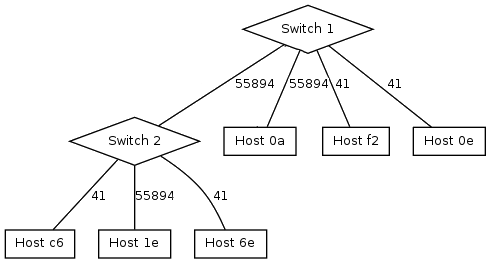
\includegraphics[scale=0.8]{img/graph-iperf}
    \caption{Tráfego TCP (em bytes) entre os hosts ’Host 1e’ e ’Host 0a’}
    \label{fig:iperf}
\end{figure}

A variação na largura de banda e vazão da rede em função da sobrecarga de 
pacotes geradas pelo \emph{host\_tracker} foi medido reduzindo o intervalo
de sondagem de computadores e efetuando a medição com \emph{iperf}. 

